\subsection{Transversal wave equation for beam elements}
\label{subsec:transversal_wave_equation_beam_elements}

To recall the transversal wave equation for beam elements, we start by considering the equilibrium of forces acting on an infinitesimal element of the beam, as shown in Figure \ref{fig:beam_element_forces}.
We assume here small displacements and rotations, linear elastic material behavior (isotropic), homogeneous material properties, negligible damping, slender beam, and no tension or compression forces applied.

One can also recognize that these assumptions are similar to the ones made in the Euler-Bernoulli beam theory.
Thanks to the EB theory, we can also assume that the angular distortion produced in the beam by the action of shear forces is negligible and that the effect of rotational inertia is also negligible.
Based on these last assumptions, the following relation between the transversal displacement $w(x,t)$ and the bending moment $M(x,t)$ is obtained:

\begin{equation}
    M(x,t) = -EJ \frac{\partial^2 w(x,t)}{\partial x^2}
    \label{eq:bending_moment_transversal_displacement}
\end{equation}

Where $E$ is the Young's modulus, $J$ is the moment of inertia of the beam section, and $x$ is the coordinate along the beam axis.

\begin{figure}[H]
    \centering

    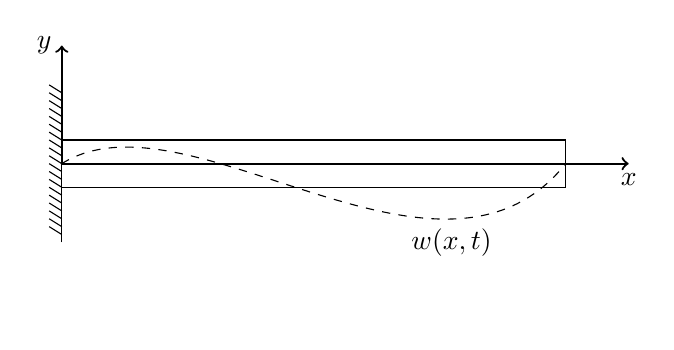
\begin{tikzpicture}[xscale=0.8]

        \draw (0, -0.3) rectangle (8, 0.3);

        \draw[->, thick] (0, 0) -- ++(9, 0) node[below]{$x$};
        \draw[->, thick] (0, 0) -- ++(0, 1.5) node[left]{$y$};
        \draw (0, -1) -- (0,  1);
        \draw[dashed] (0,0) .. controls (2, 1) and (6, -2) .. (8, 0) node[pos=0.75, below]{$w(x,t)$};

        \foreach \y in {-0.9, -0.8, ..., 0.9}
        \draw (0, \y) -- ++(-0.2, +0.1);

    \end{tikzpicture}
    \hspace{1cm}
    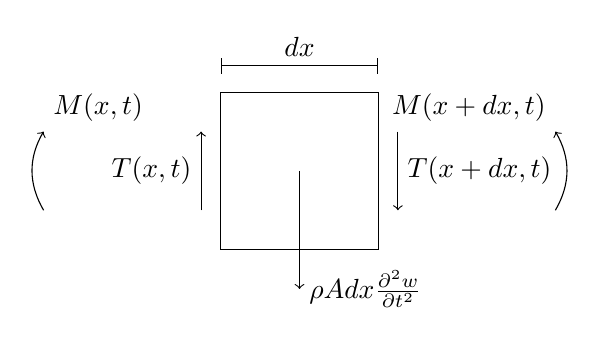
\begin{tikzpicture}

        \def\dx{2}
        \def\dy{2}

        \draw[|-|] (-\dx/2, +4/3*\dy/2) -- ++(\dx, 0) node[midway, above]{$dx$};

        \draw (-\dx/2, -\dy/2) rectangle (\dx/2, \dy/2);
        \draw[->] (0, 0) -- ++(0, -3/4*\dy) node[right]{$\rho A dx\frac{\partial^2 w}{\partial t^2}$};
        \draw[->] (-5/4*\dx/2, -\dy/4) -- ++(0, +1) node[midway, left]{$T(x, t)$};
        \draw[->] (+5/4*\dx/2, +\dy/4) -- ++(0, -1) node[midway, right]{$T(x + dx, t)$};
        \draw[->] (-13/4*\dx/2, -\dy/4) to [bend left] (-13/4*\dx/2, +\dy/4) node[above right]{$M(x, t)$};
        \draw[->] (+13/4*\dx/2, -\dy/4) to [bend right] (+13/4*\dx/2, +\dy/4) node[above left]{$M(x + dx, t)$};

    \end{tikzpicture}

    \caption{Transversal displacement $w(x,t)$ of a beam element and forces acting on infinitesimal element ($dx$).}
    \label{fig:beam_element_forces}

\end{figure}

Using D'Alambert principle, we can write the following vertical and rotational equilibrium for the infinitesimal element represented in Figure \ref{fig:beam_element_forces}:

\begin{equation}
    \begin{matrix}
        -M(x,t) + M(x + dx, t) - T(x,t) \frac{dx}{2} - T(x + dx, t) \frac{dx}{2} = 0 \\
        T(x, t) - T(x + dx, t) = \rho A dx \frac{\partial^2 w}{\partial t^2}
    \end{matrix}
\end{equation}

Using differential calculus, we can rewrite this equilibrium as:

\begin{equation}
    \begin{matrix}
        -M(x,t) + M(x, t) + \frac{\partial M(x,t)}{\partial x} dx - T(x,t) \frac{dx}{2} - T(x,t) \frac{dx}{2} - \frac{\partial T(x,t)}{\partial x} \frac{dx^2}{2} = 0 \\
        T(x, t) - T(x, t) - \frac{\partial T(x, t)}{\partial x} dx = \rho A dx \frac{\partial^2 w}{\partial t^2}
    \end{matrix}
\end{equation}

From which (neglecting higher order terms) we obtain:

\begin{equation}
    \begin{aligned}
        T(x, t)                            & = \frac{\partial M(x,t)}{\partial x}              \\
        \frac{\partial T(x,t)}{\partial x} & = - \rho A \frac{\partial^2 w(x,t)}{\partial t^2}
    \end{aligned}
\end{equation}

Substituting the expression of $T(x,t)$ and recalling the definition of $M(x, t)$ (see Equation \ref{eq:bending_moment_transversal_displacement}), we obtain the following equation of motion for the transversal displacement $w(x,t)$:

\begin{equation}
    \frac{\partial^2}{\partial x^2} \left( EJ \frac{\partial^2 w(x,t)}{\partial x^2} \right) = -\rho A \frac{\partial^2 w(x,t)}{\partial t^2}
    \label{eq:beam_equation_of_motion_transversal_displacement}
\end{equation}

It's easy to recognize that Equation \ref{eq:beam_equation_of_motion_transversal_displacement} is a fourth-order partial differential equation (PDE) in the space variable $x$ and a second-order PDE in the time variable $t$.

In case the material properties are constant both in time and space, $w(x,t)$ can be computed analytically as the product of a spatial function $\alpha(x)$ and a temporal function $\beta(t)$.
However, in the case of non-constant material properties, the problem becomes more complex and numerical methods are usually required to solve it.
